\chapter{Repository and Contribution Evidence}
\label{app:repo}
\section{Pull requests}
\begin{table}[H]
\centering\small
\begin{tabular}{p{0.05\textwidth}p{0.47\textwidth}p{0.18\textwidth}p{0.18\textwidth}}
\toprule
\# & Title & Base & CI\\
\midrule
1 & CI/CD pipeline, unit tests, containers and FYP scope & \code{develop} & Frontend 44\,s pass; Backend 2\,m\,20\,s pass\\
2 & Phase 10 backend: score explanations, alerts, paper book, health, product state & \#1 & Frontend pass; Backend pass\\
3 & Product rework: anatomy, push, paper book, model health, persistence; cuts per scope & \#2 & Frontend pass; Backend pass\\
4 & CI hardening: end-to-end tests, audits, coverage floors, staging tag, image scan & \#3 & Frontend, Backend, End to end pass; Audit failed on Starlette 0.48, fixed by upgrade\\
\bottomrule
\end{tabular}
\caption{Pull requests at the time of writing. \todo{Add screenshots of the merged PRs and the Actions page before submission.}}
\end{table}
\section{Branch model}
\begin{lstlisting}
main      <- release pull requests from develop; CD publishes :latest and releases on v* tags
develop   <- squash-merged feature pull requests; CD publishes :develop (staging)
feature/* <- one piece of work each; CI on every push and pull request
\end{lstlisting}
\section{Screenshots}
\begin{figure}[H]\centering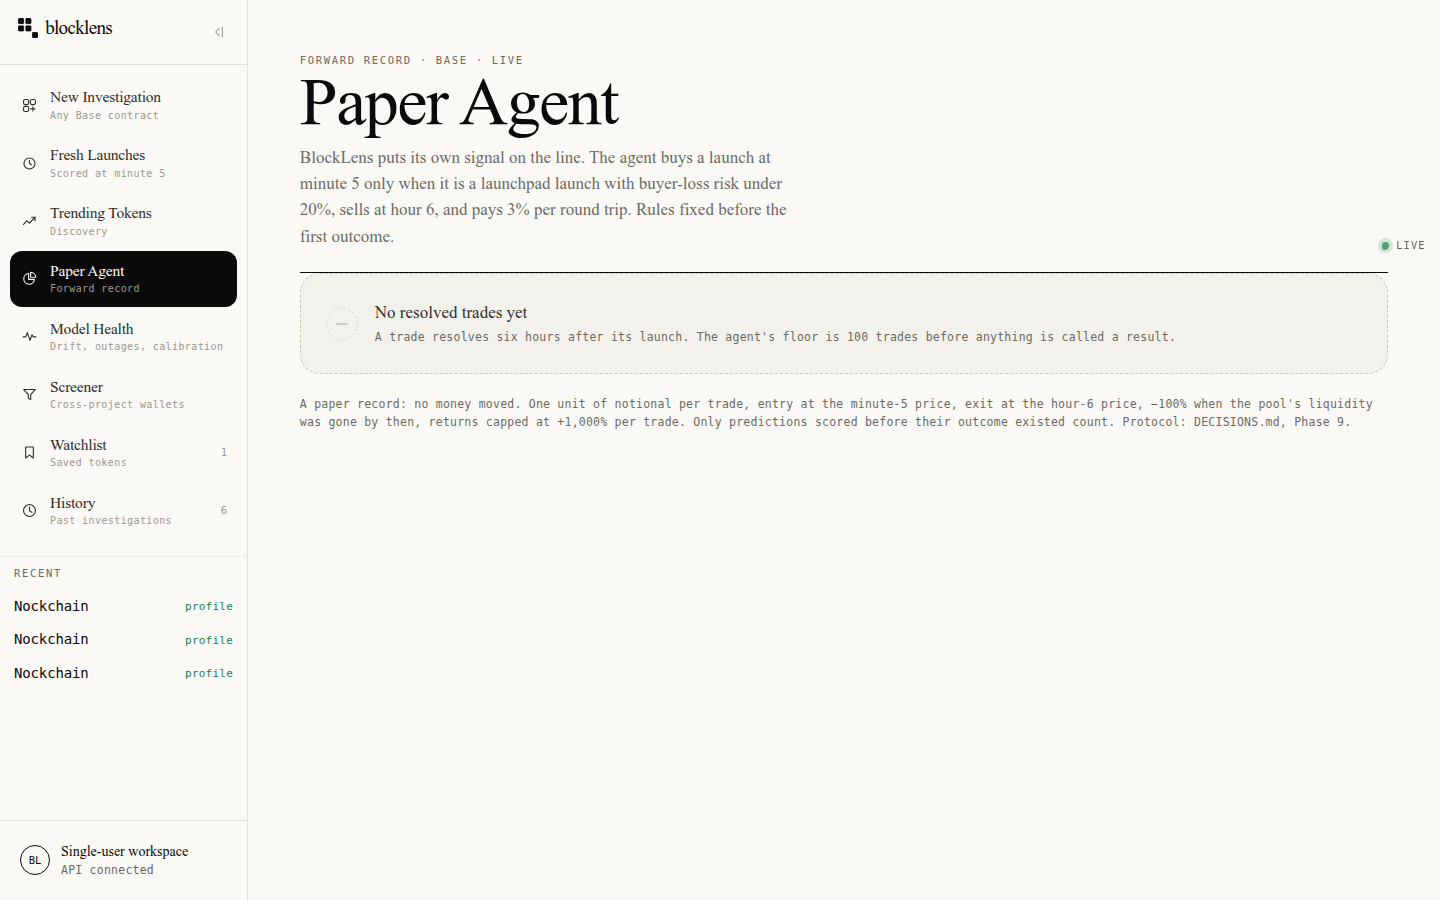
\includegraphics[width=\textwidth]{figures/portfolio.png}\caption{Paper Agent page (empty state on a fresh store; the live deployment shows the 850-trade book).}\end{figure}
\begin{figure}[H]\centering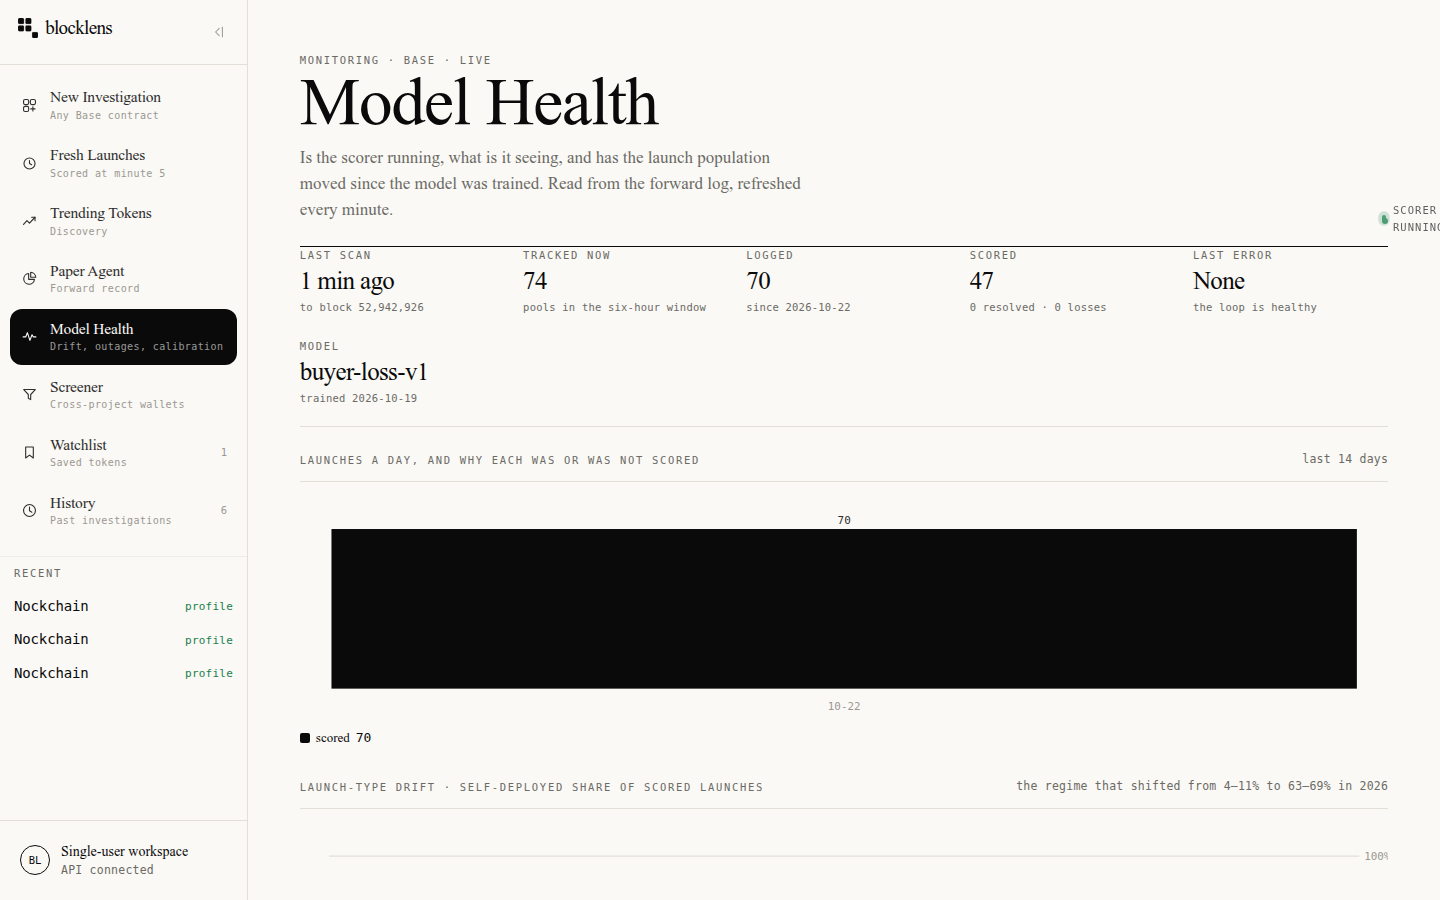
\includegraphics[width=\textwidth]{figures/model.png}\caption{Model Health page.}\end{figure}
\begin{figure}[H]\centering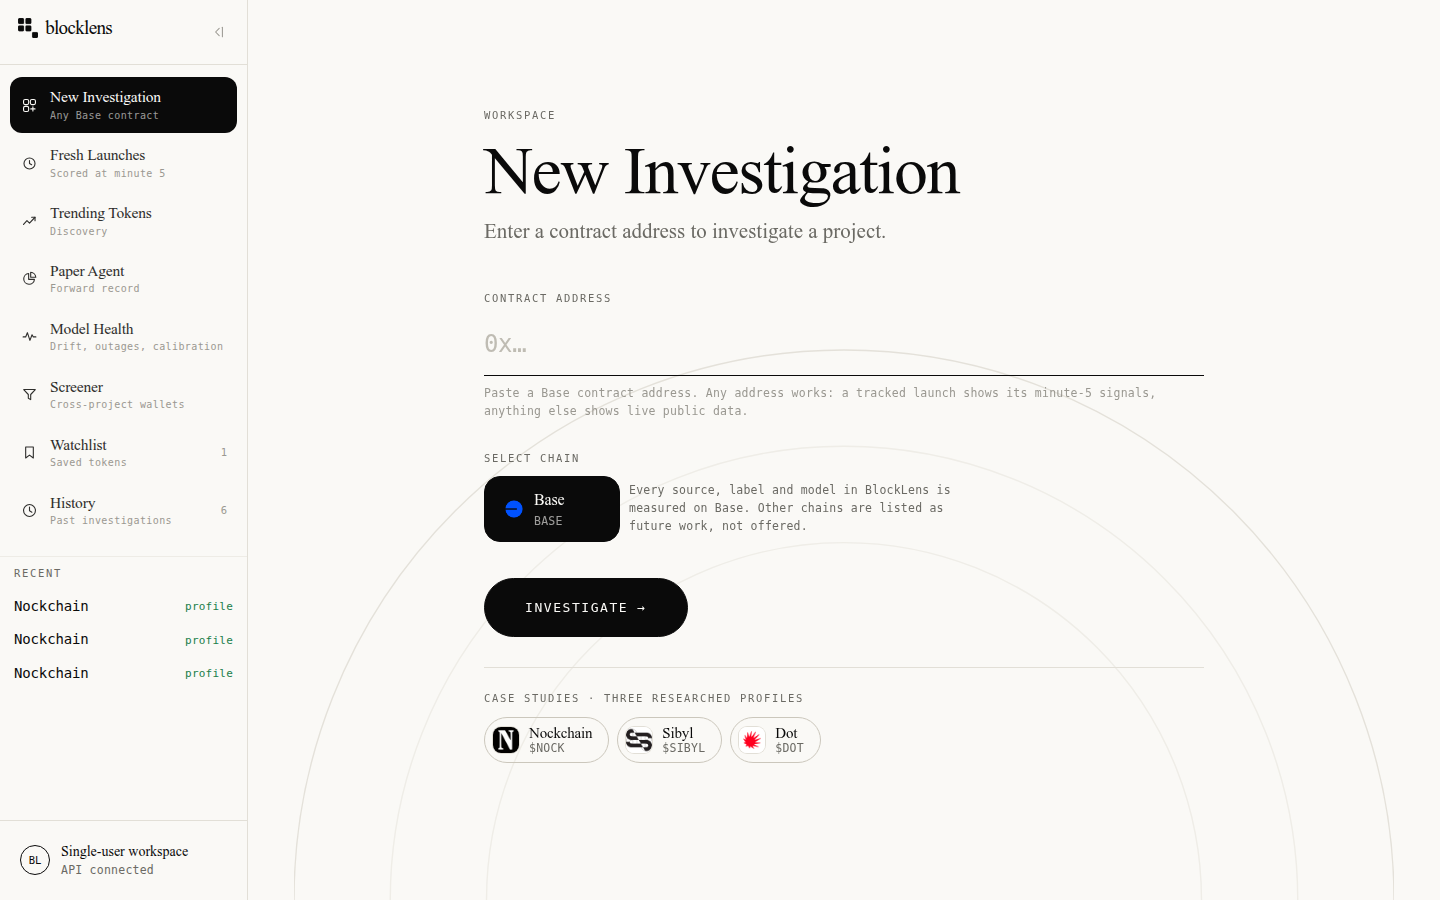
\includegraphics[width=\textwidth]{figures/new.png}\caption{New Investigation: any Base address; the three case studies offered as such.}\end{figure}
\begin{figure}[H]\centering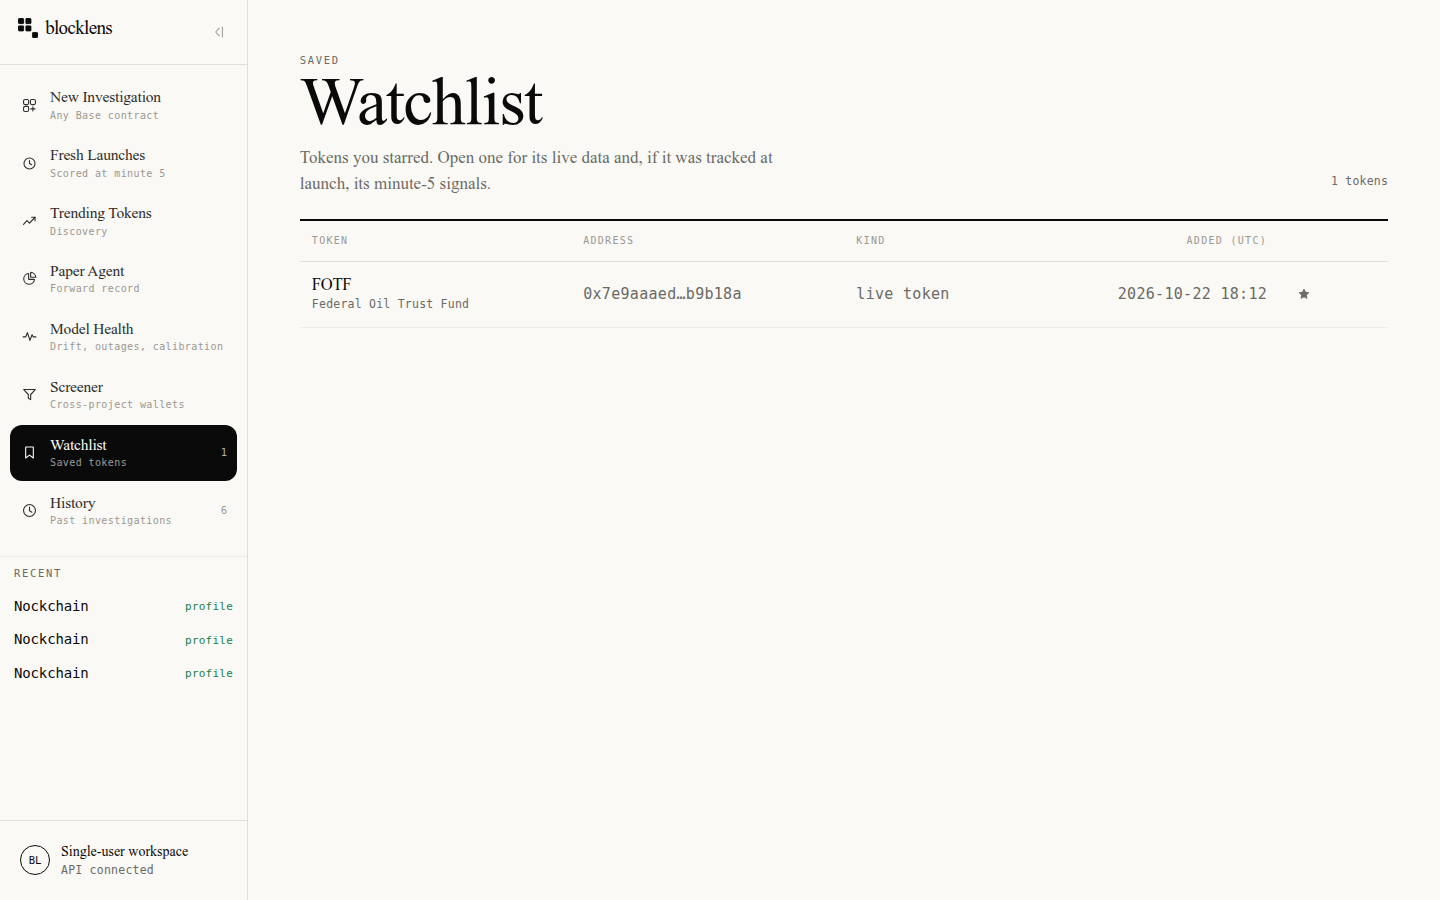
\includegraphics[width=\textwidth]{figures/watchlist.png}\caption{Watchlist held by the API.}\end{figure}
\todo{Add: a screenshot of the GitHub Actions run list and of one green pull request.}
